% Appendix A

\chapter{Plànols de les peces} % Main appendix title

\label{AppendixB} % For referencing this appendix elsewhere, use \ref{AppendixA}

\lhead{} % This is for the header on each page - perhaps a shortened title
\rhead{}

\textbf{B.1 Xassís}\\

\textbf{B.2 Guia del retolador}\\

\textbf{B.3 Mecanisme d'elevació del retolador}\\

\textbf{B.4 Roda boja davantera}\\

\textbf{B.5 Roda motriu}\\

\textbf{B.6 Tubs auxiliars}\\




\clearpage\pagestyle{empty}
\section{Xassís} 
\begin{picture} (0,0)
	\put(-82,-722){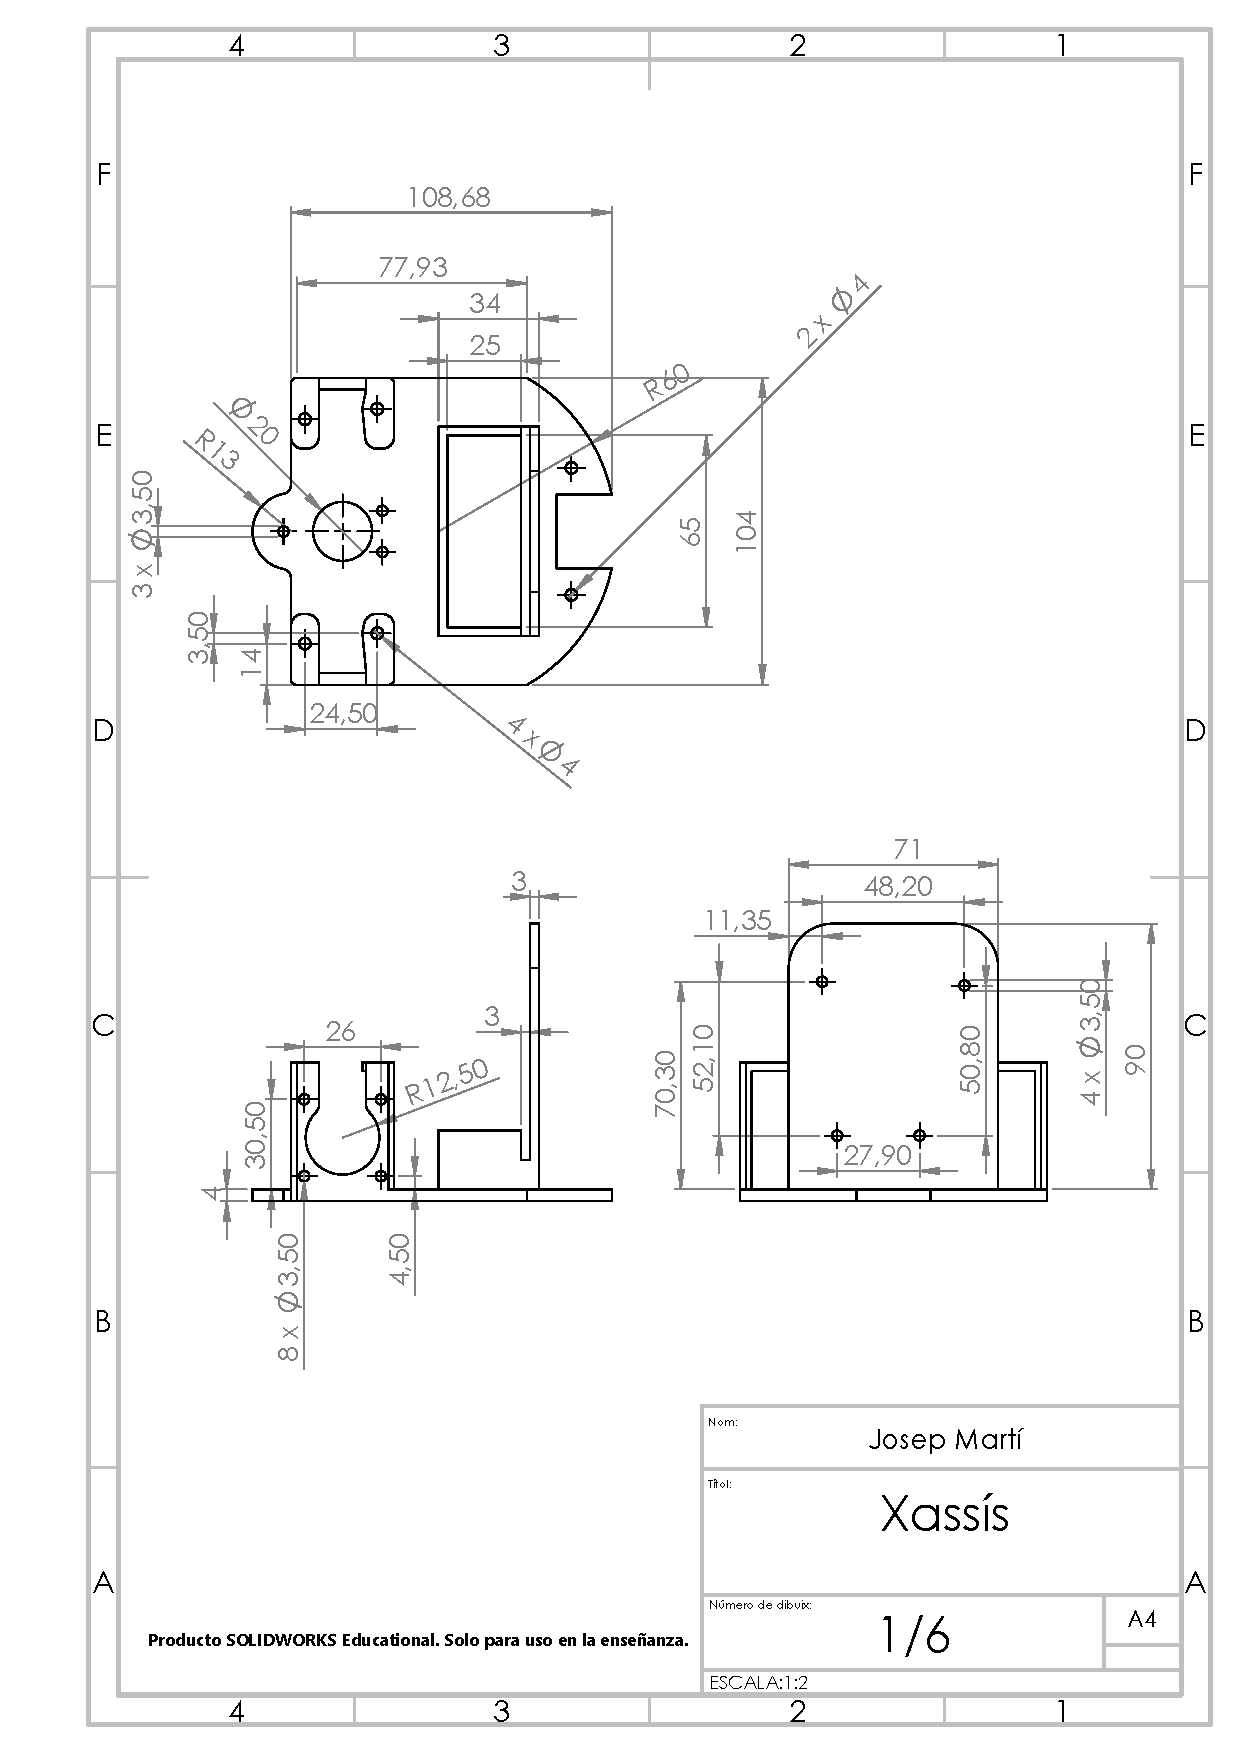
\includegraphics{XassisPlanol}}
\end{picture}

\clearpage\pagestyle{empty}
\section{Guia del retolador} 
\begin{picture} (0,0)
\put(-105,-722){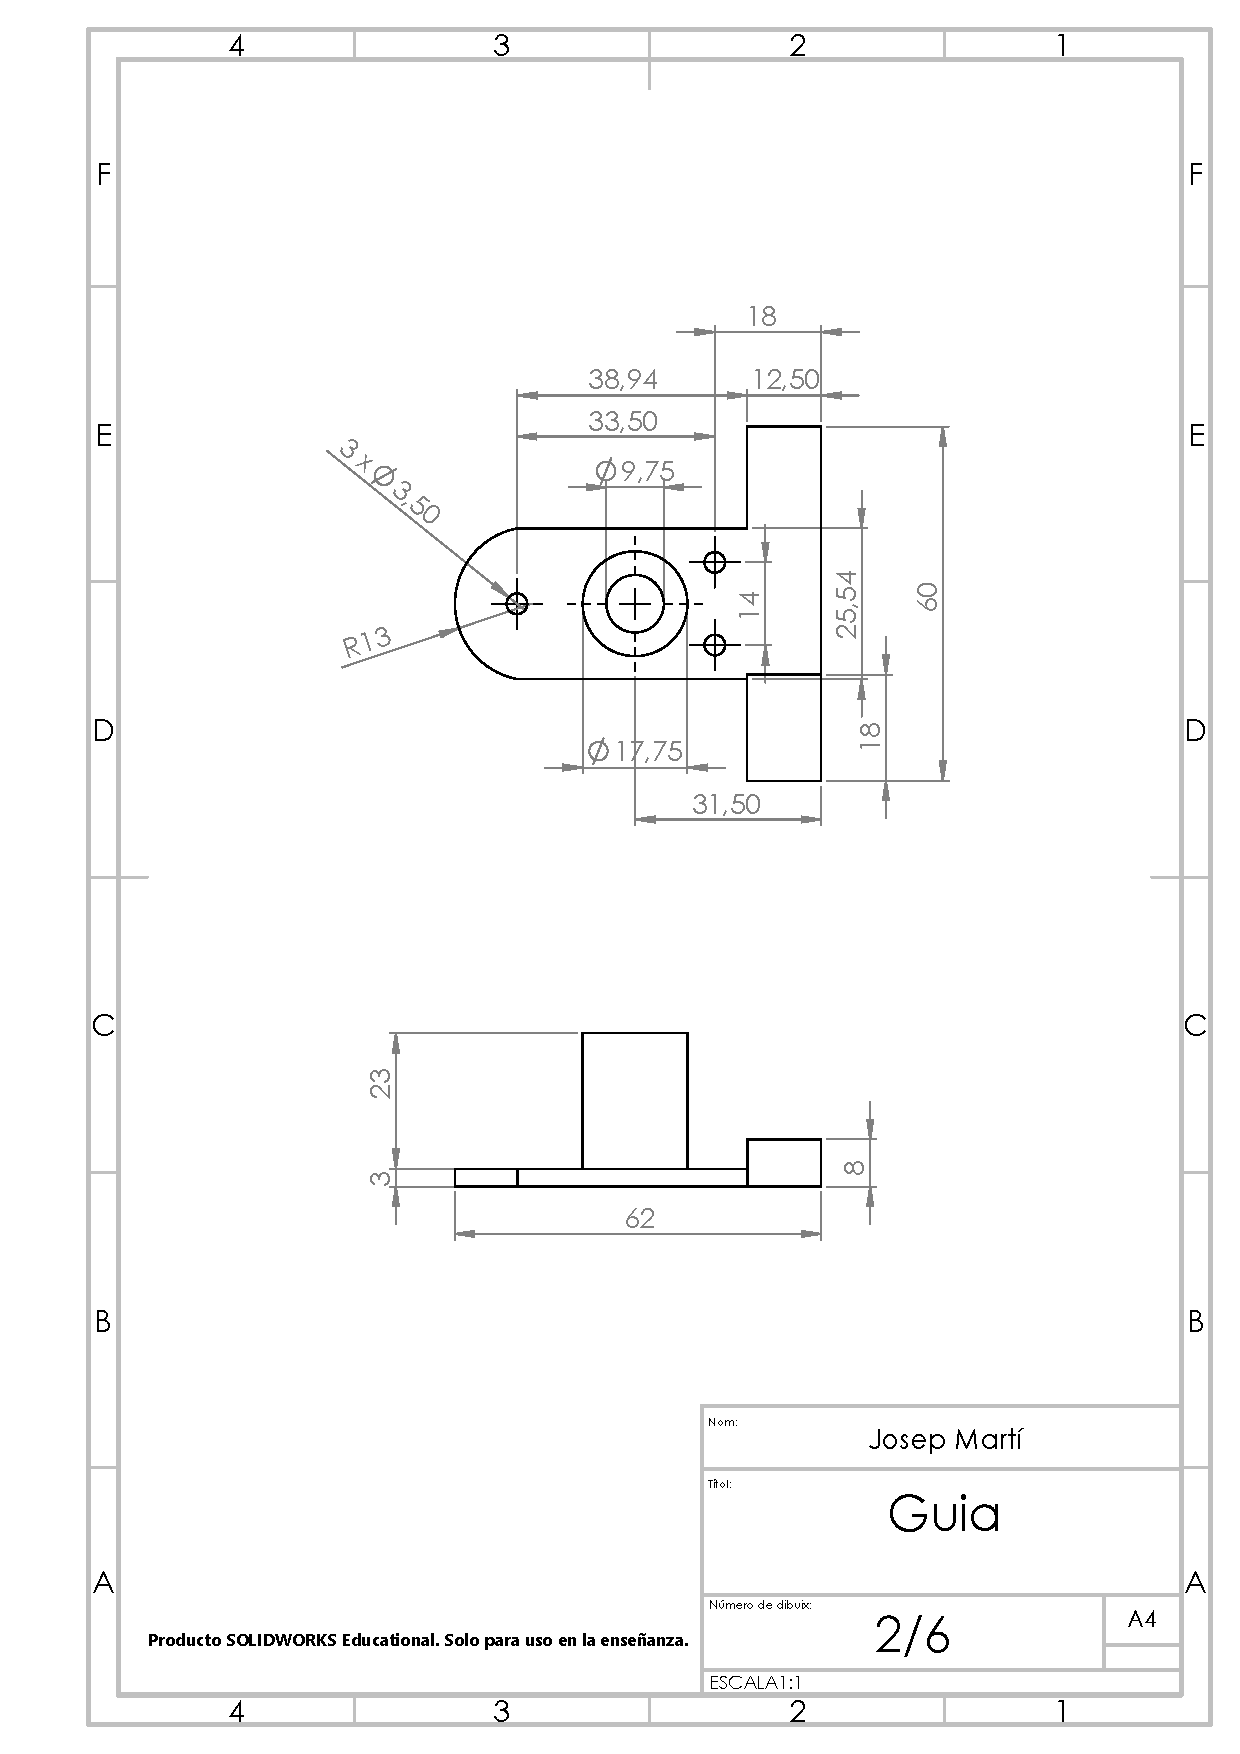
\includegraphics{GuiaPlanol}}
\end{picture}

\clearpage\pagestyle{empty}
\section{Mecanisme d'elevació del retolador} 
\begin{picture} (0,0)
\put(-82,-722){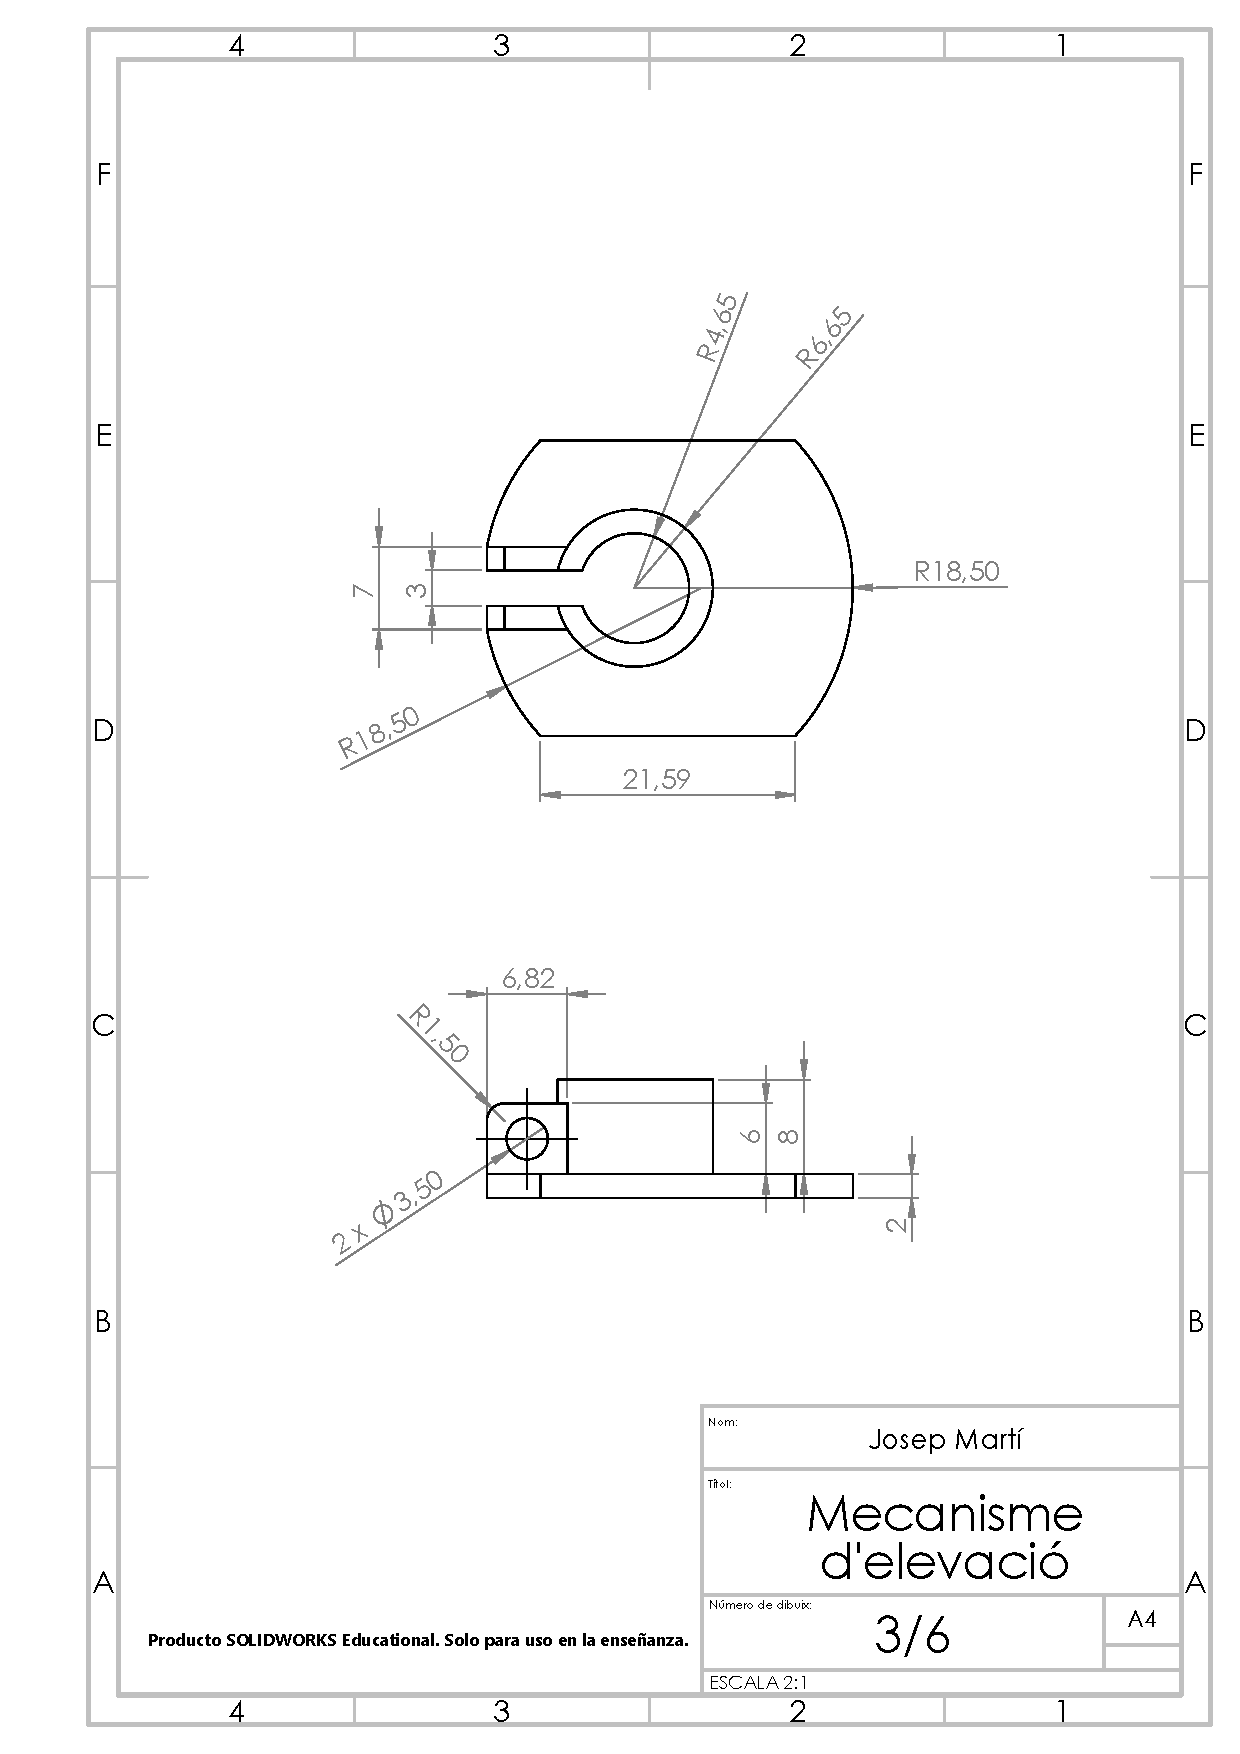
\includegraphics{SuportPlanol}}
\end{picture}

\clearpage\pagestyle{empty}
\section{Roda boja davantera} 
\begin{picture} (0,0)
\put(-105,-722){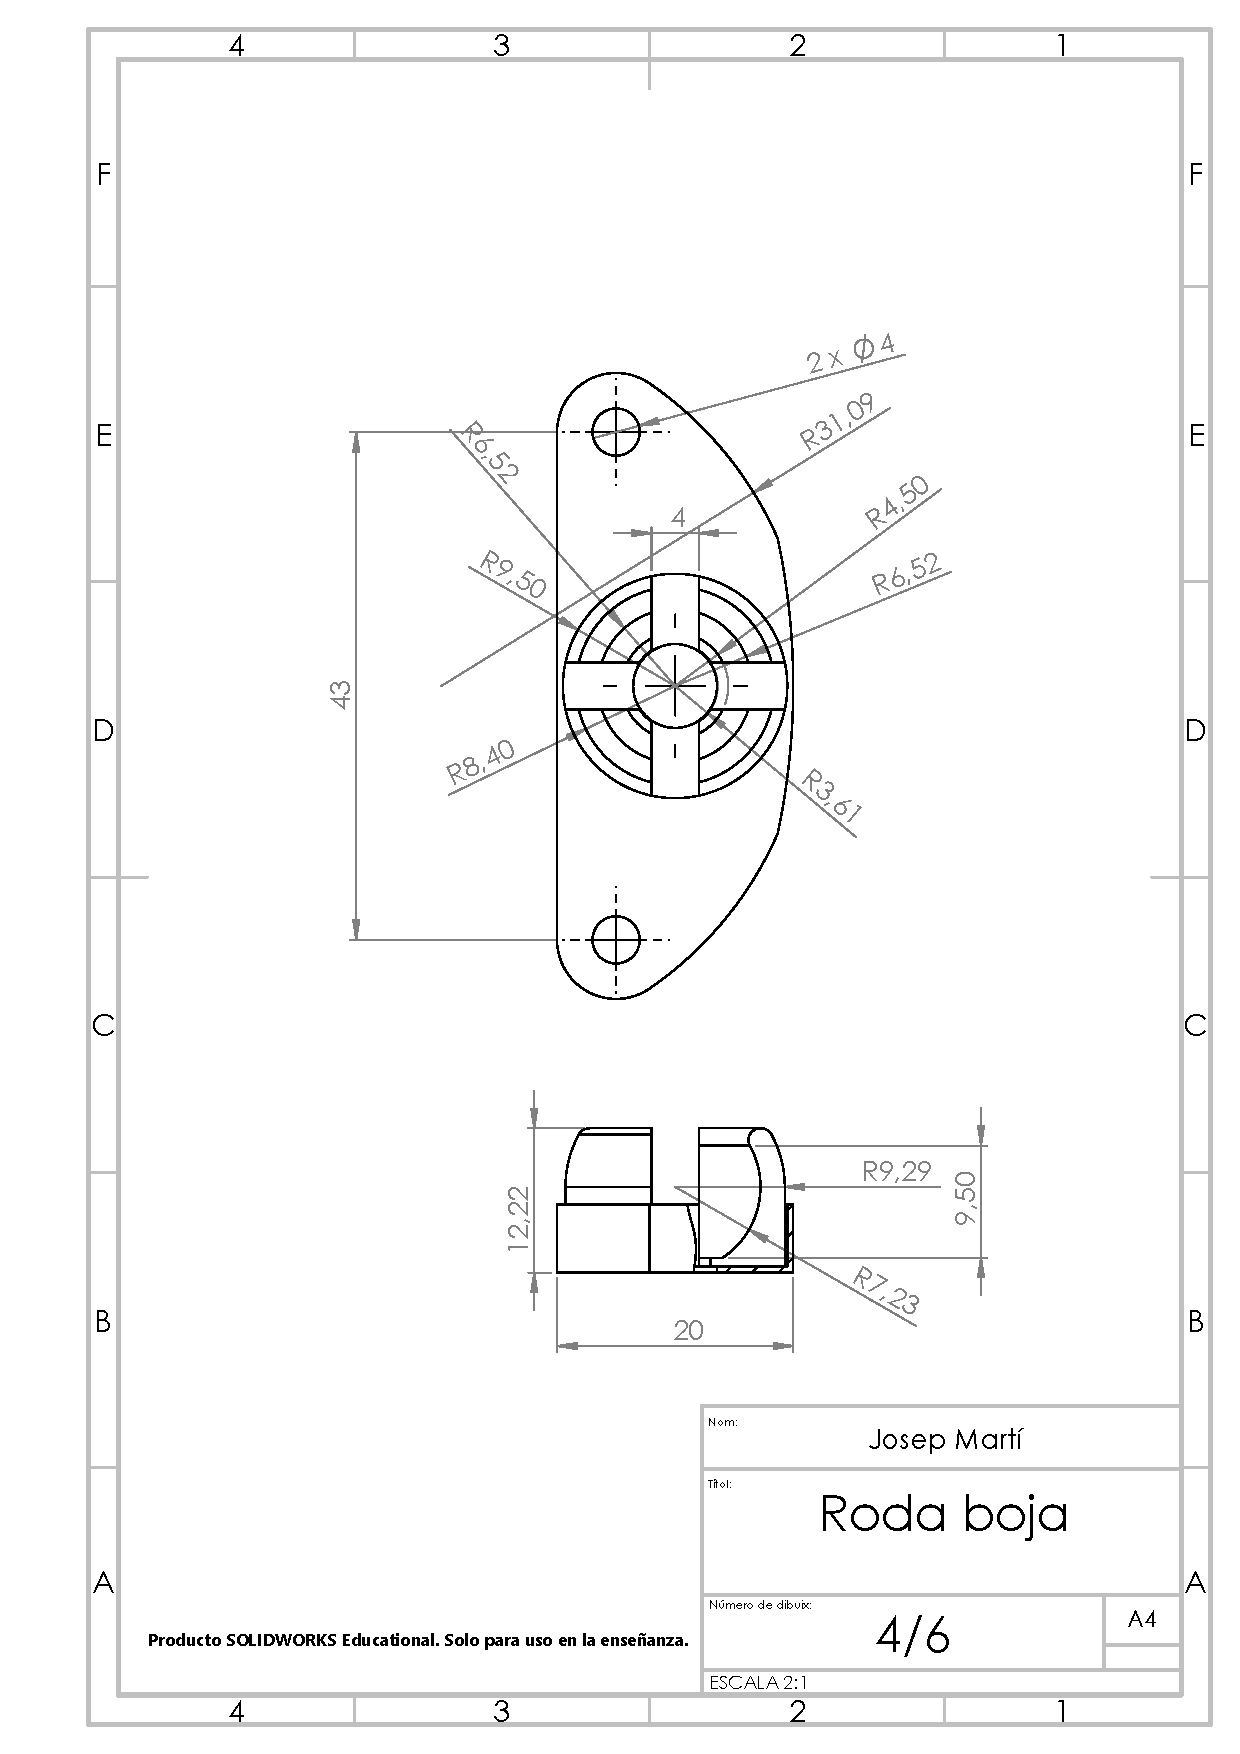
\includegraphics{RodaBojaPlanol}}
\end{picture}

\clearpage\pagestyle{empty}
\section{Roda motriu} 
\begin{picture} (0,0)
\put(-82,-722){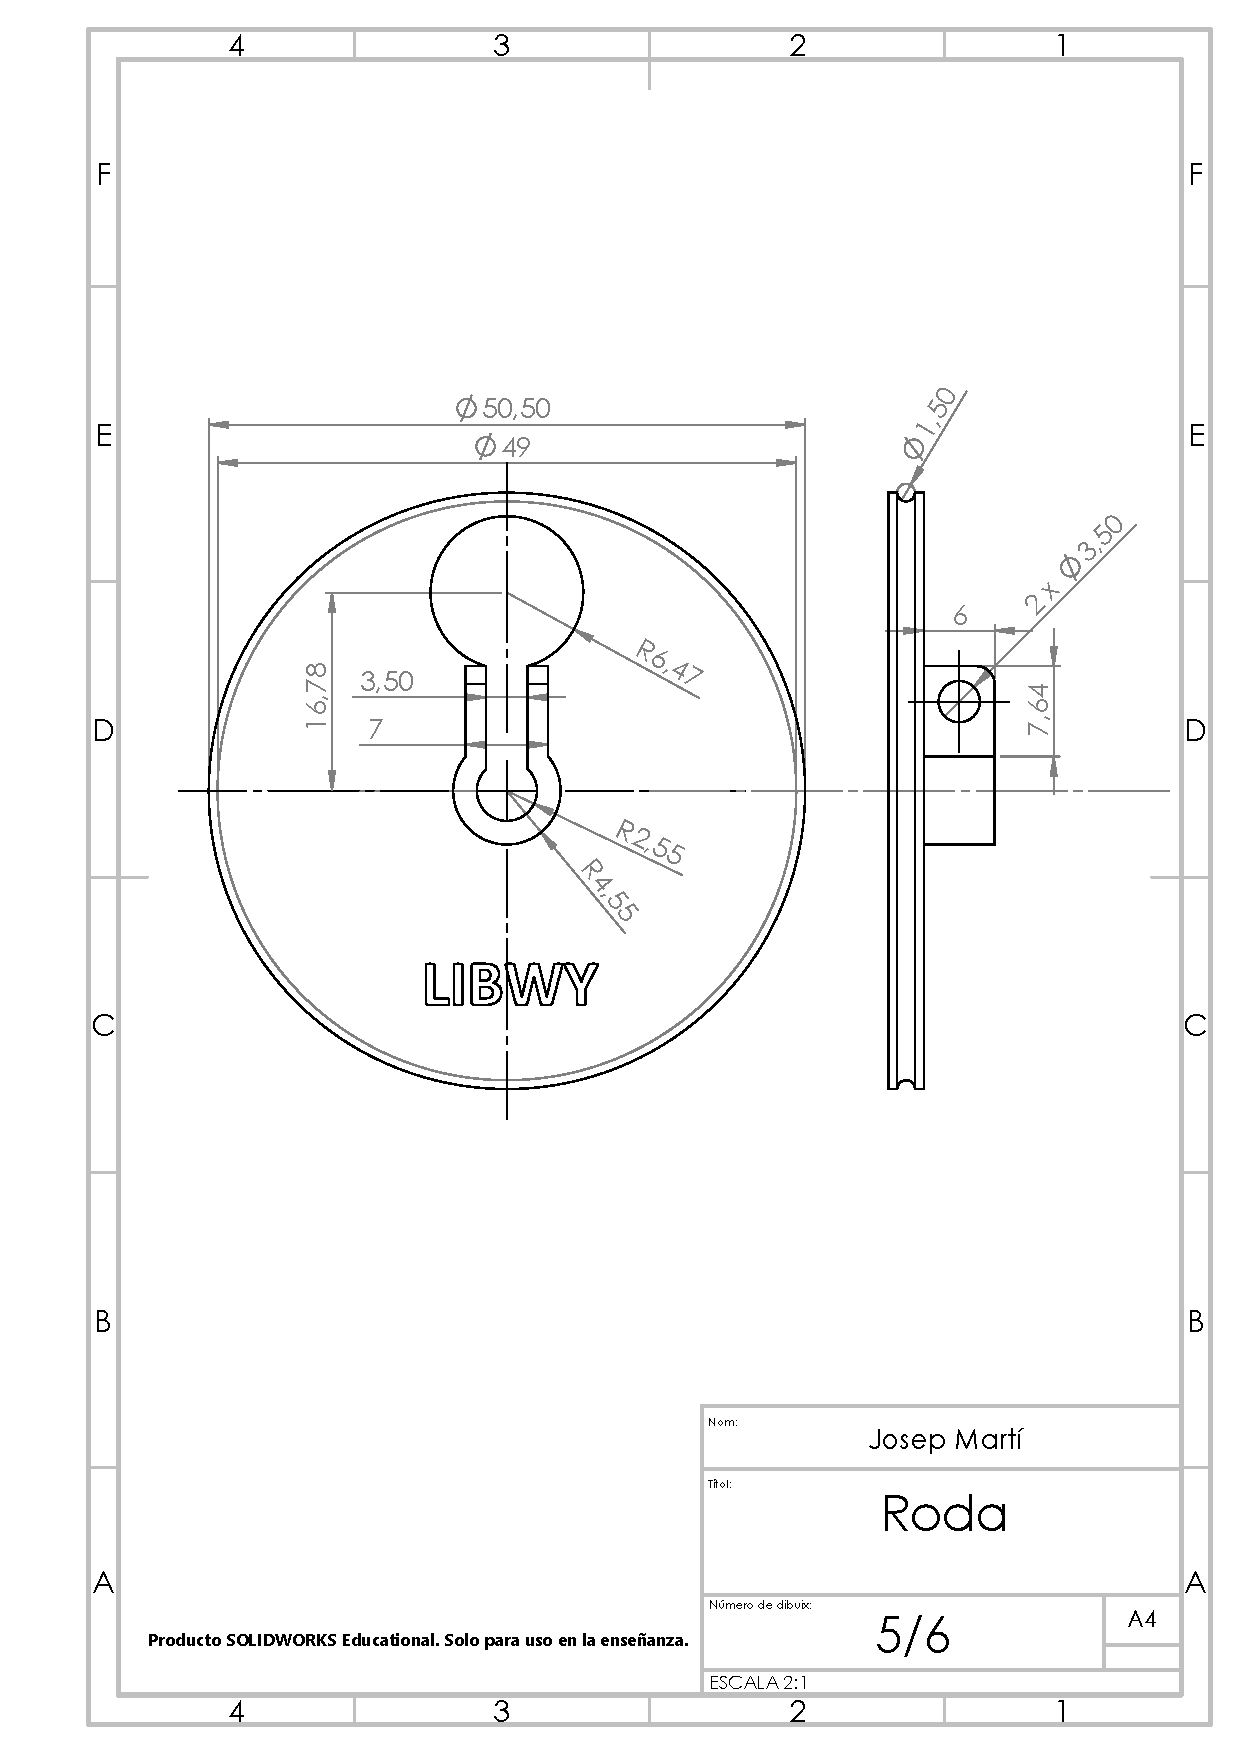
\includegraphics{RodaPlanol}}
\end{picture}

\clearpage\pagestyle{empty}
\section{Tubs auxiliars} 
\begin{picture} (0,0)
\put(-105,-722){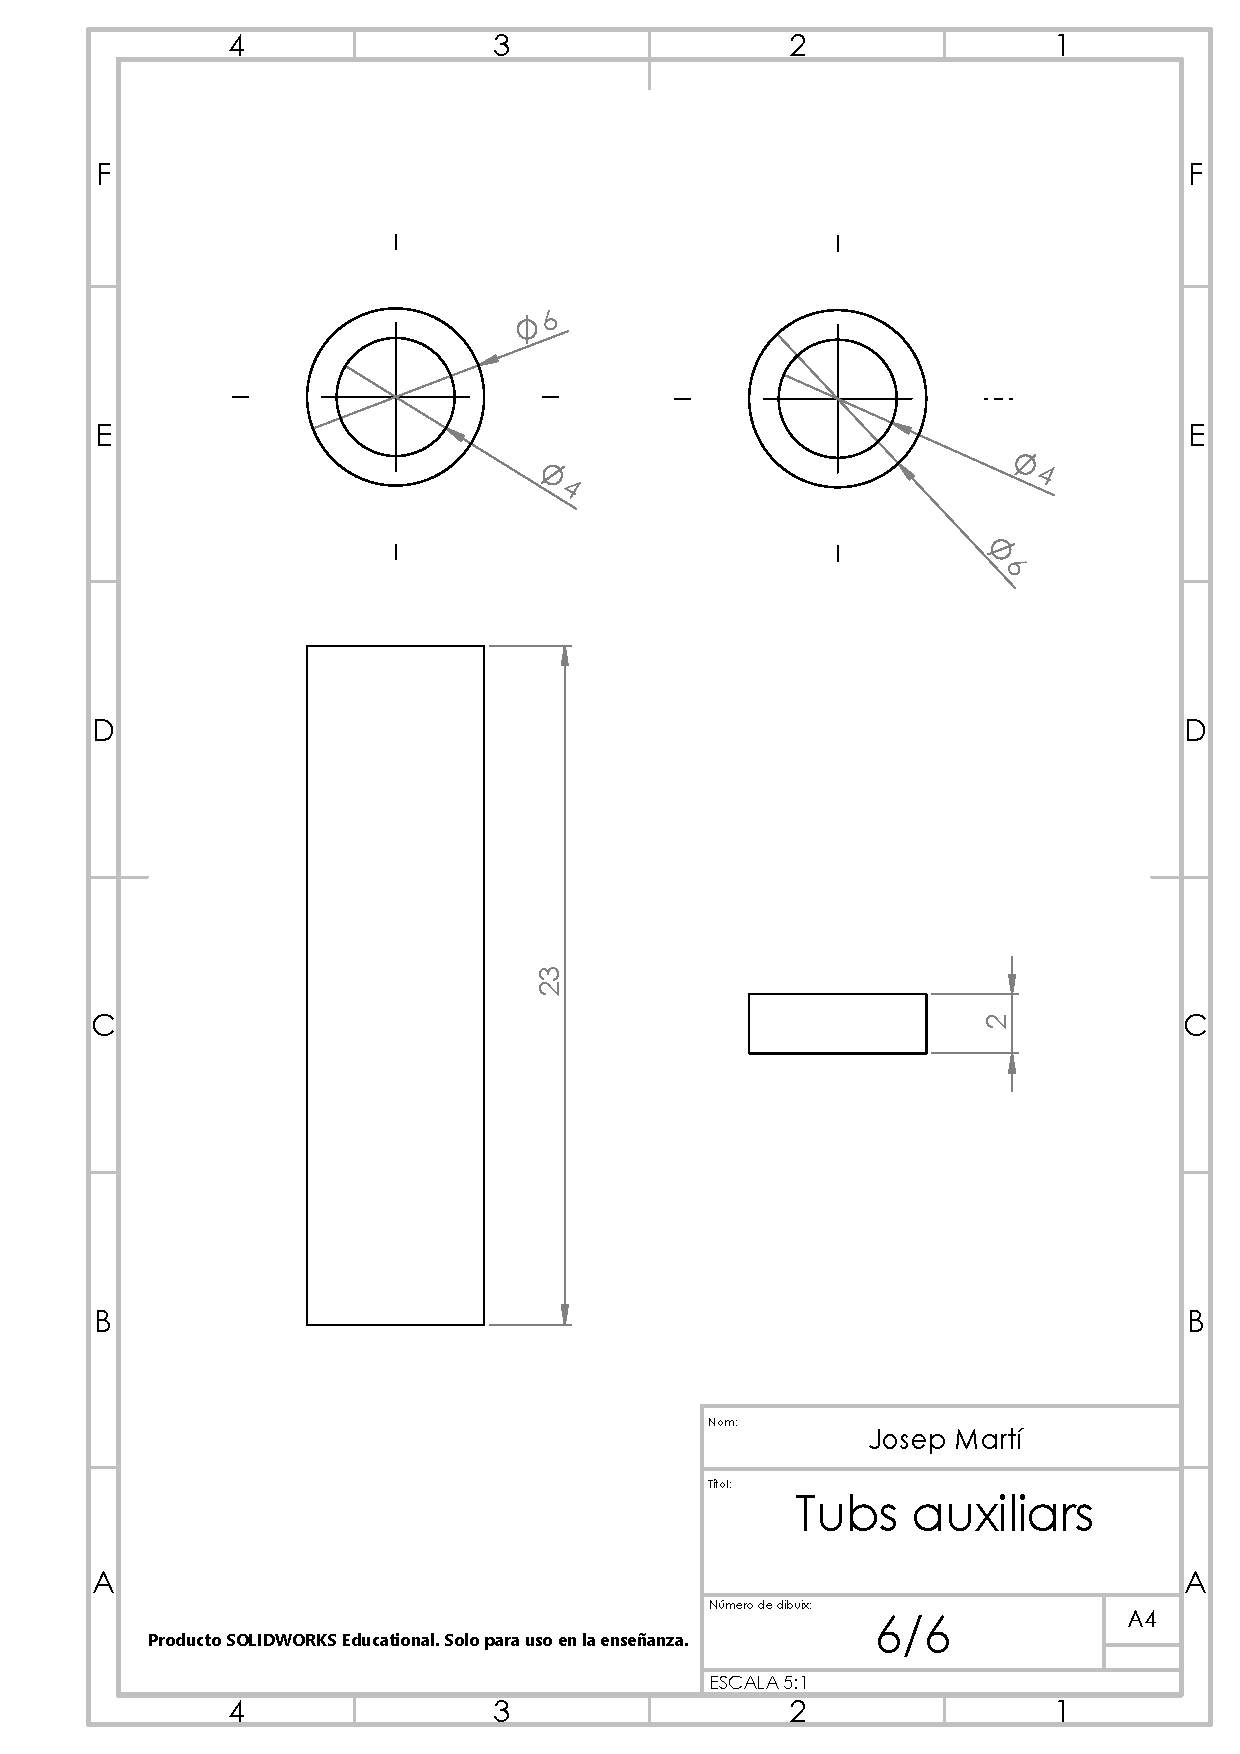
\includegraphics{TubsPlanol}}
\end{picture}

%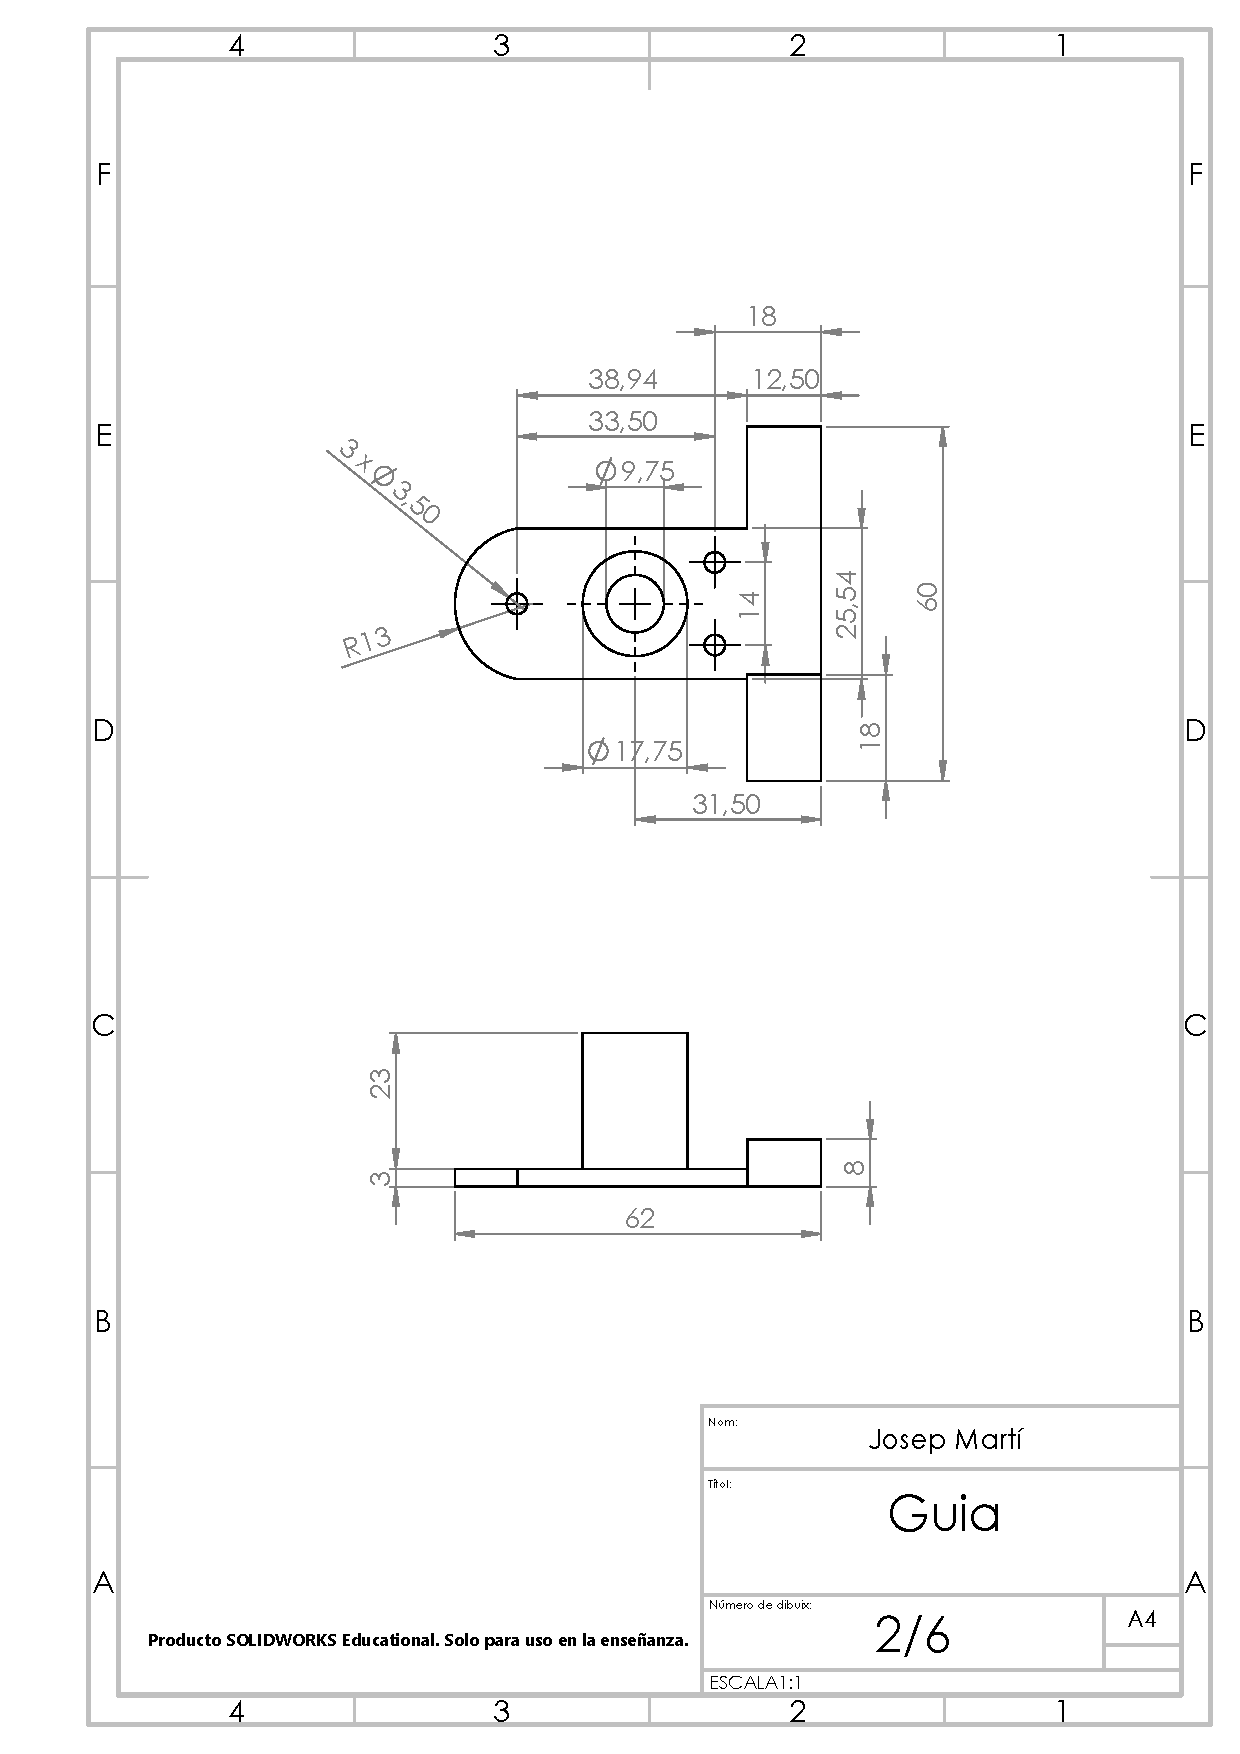
\includepdf[page={1},fitpaper=true, trim=0mm 0mm 0mm 0mm, clip]{GuiaPlanol}